\chapter{3+1 Formalism}

The 3+1 formalism is a method in general relativity, where we slice the spacetime manifold into a foliation of Cauchy hypersurfaces (three-dimensional surfaces). 
Due to the metric induced by the Lorentzian spacetime metric needing to be Riemannian, the hypersurfaces are required to be spacelike.
From a naïve point of view, this can be seen as a decomposition from spacetime into "space" + "time". It should be noted this spliting requires a well established and concise choice of time coordinate.

This formalism is also useful for solving the initial value problem, with this decomposition, solving the Einstein equation is equivalent to solving a Cauchy problem.

Studies with the 3+1 formalism started in the 1920s by Georges Darmois and continued until the 1950s, by direct affiliations. In 1952, Yvonne Choquet-Bruhat verified that the Cauchy problem, arising from the 3+1 decomposition has locally a unique solution \cite{}.
Later in the decade, Dirac motivated a similar formalism, based on an Hamiltonian approach, which later was called ADM, by Arnowitt, Deser and Misner\cite{}. Around the same time, Wheeler introduced the concept of geometrodynamics and coined the terms, soon mentioned, "lapse" and "shift". 
In the 1970s, the 3+1 formalism became an essential tool, to numerical relativity.

In this chapter, we will be only considering a single general fluid.

\section{Description of the geometry}

Let us consider a four-dimensional manifold, $\mathcal{M}$, with a Lorentzian metric tensor $\mathbf{g}$ and described under a local coordinate system $x^\mu=(y,x^i)$, where $\mathbf{g}=g_{\mu\nu}dx^\mu \otimes dx^\nu$. 
In this spacetime, matter is described by a matter content fluid, where the fluid flow is described by a timelike congruence with a unit, future-oriented, timelike tangent four-vector field $\mathbf{u}$, describing its four-velocity. 
Meanwhile we will not make any exact physical interpretation on this four-velocity\footnote{The four-velocity could be a energy frame of the fluid, a barycentric velocity, or the unit vector associated to another conserved current.}.

The foliation is performed by slicing $\mathcal{M}$ in a family $y=\text{const}$ hypersurfaces which we denote $\Sigma_y$. 
Locally these hypersurfaces will share the same topology $\Sigma_y \simeq \Sigma$. 
Therefore locally we have $\mathcal{M}\simeq \mathbb{R}\times \Sigma$. 
And we denote by $\mathbf{n}$ their unit, future-oriented and timelike normal vector field, which generally is tilted with respect to the four-velocity $\mathbf{u}$.
And we denote by $\bm{\partial_y}$ the vector parallel to the motion along $y$, when the $x^i$ are held fixed.
We can characterize this foliation by a scalar function $y$ restrictively increasing along each flow line, and defined in such a way that each hypersurface is a level set of $y$. For the time being we choose the time coordinate $t$, as this stricly increasing function, implying that $y\equiv y(t)$. 


\begin{figure}[ht]
    \centering

\tikzset{every picture/.style={line width=0.75pt}} %set default line width to 0.75pt        

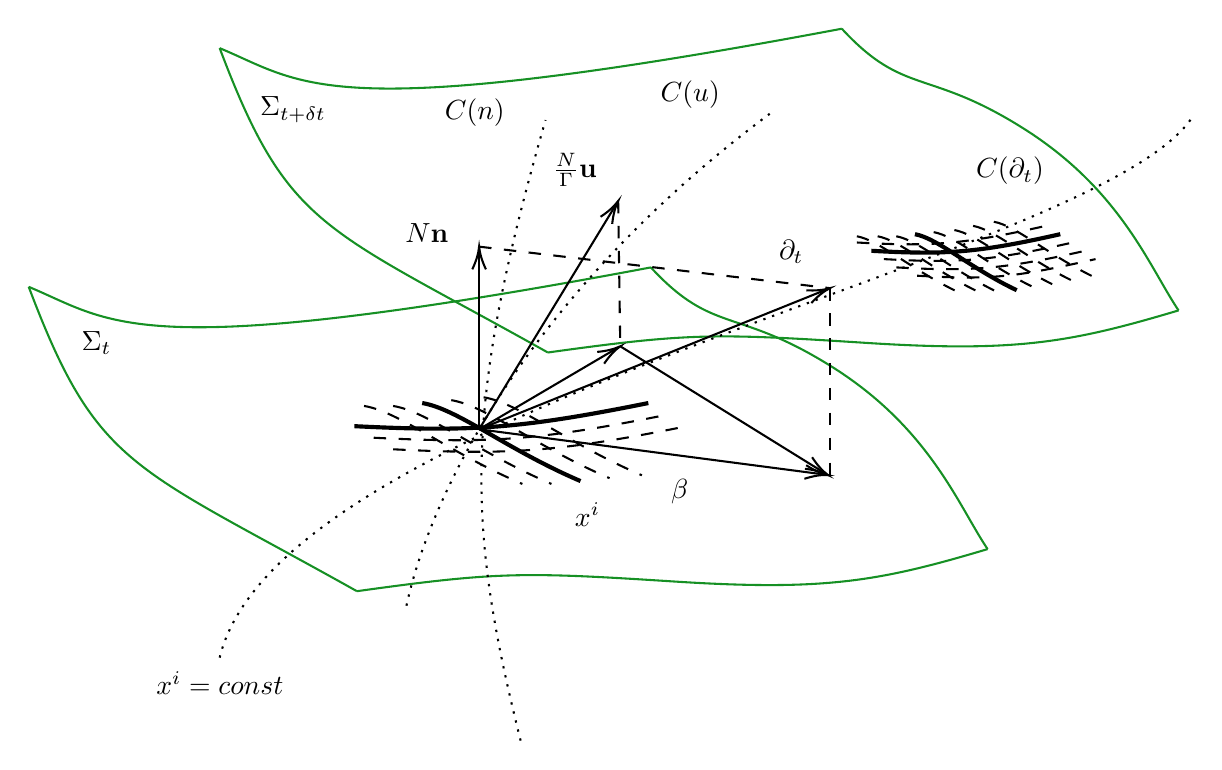
\begin{tikzpicture}[x=0.75pt,y=0.75pt,yscale=-1,xscale=1]
%uncomment if require: \path (0,467); %set diagram left start at 0, and has height of 467

%Curve Lines [id:da13576815661454944] 
\draw [color={rgb, 255:red, 22; green, 144; blue, 36 }  ,draw opacity=1 ]   (48,205.36) .. controls (81,292.72) and (97.5,291.16) .. (206.12,352) ;
%Curve Lines [id:da3389506239015292] 
\draw [color={rgb, 255:red, 22; green, 144; blue, 36 }  ,draw opacity=1 ]   (206.12,352) .. controls (273.5,342.64) and (285.88,342.64) .. (358.75,347.32) .. controls (431.63,352) and (457.75,347.32) .. (510,331.72) ;
%Curve Lines [id:da2722842924714688] 
\draw [color={rgb, 255:red, 22; green, 144; blue, 36 }  ,draw opacity=1 ]   (347.75,196) .. controls (378,228.76) and (389,214.72) .. (435.75,244.36) .. controls (482.5,274) and (496.25,311.44) .. (510,331.72) ;
%Curve Lines [id:da2654170172814696] 
\draw [color={rgb, 255:red, 22; green, 144; blue, 36 }  ,draw opacity=1 ]   (48,205.36) .. controls (89.25,222.52) and (98.88,242.8) .. (347.75,196) ;

%Curve Lines [id:da188980808953499] 
\draw [line width=1.5]    (204.9,272.49) .. controls (260.93,275.27) and (284.28,273.88) .. (346.54,261.35) ;
%Curve Lines [id:da33296466436615946] 
\draw  [dash pattern={on 4.5pt off 4.5pt}]  (223.57,283.63) .. controls (279.61,286.41) and (302.96,285.02) .. (365.22,272.49) ;
%Curve Lines [id:da646227828934764] 
\draw  [dash pattern={on 4.5pt off 4.5pt}]  (214.23,278.06) .. controls (270.27,280.84) and (293.62,279.45) .. (355.88,266.92) ;
%Curve Lines [id:da6452967318047047] 
\draw  [dash pattern={on 4.5pt off 4.5pt}]  (267.16,258.57) .. controls (284.28,261.35) and (307.63,280.84) .. (343.43,296.16) ;
%Curve Lines [id:da5657790292060159] 
\draw  [dash pattern={on 4.5pt off 4.5pt}]  (251.59,259.96) .. controls (268.71,262.75) and (292.06,282.24) .. (327.86,297.55) ;
%Curve Lines [id:da9932195493480838] 
\draw [line width=1.5]    (237.58,261.35) .. controls (254.7,264.14) and (278.05,283.63) .. (313.85,298.94) ;
%Curve Lines [id:da056229993422925784] 
\draw  [dash pattern={on 4.5pt off 4.5pt}]  (223.57,262.75) .. controls (240.7,265.53) and (264.04,285.02) .. (299.84,300.33) ;
%Curve Lines [id:da8916754691070794] 
\draw  [dash pattern={on 4.5pt off 4.5pt}]  (209.57,262.75) .. controls (226.69,265.53) and (250.03,285.02) .. (285.83,300.33) ;
%Curve Lines [id:da7913518320312014] 
\draw [color={rgb, 255:red, 22; green, 144; blue, 36 }  ,draw opacity=1 ]   (140,90.36) .. controls (173,177.72) and (189.5,176.16) .. (298.12,237) ;
%Curve Lines [id:da20504120863374542] 
\draw [color={rgb, 255:red, 22; green, 144; blue, 36 }  ,draw opacity=1 ]   (298.12,237) .. controls (365.5,227.64) and (377.88,227.64) .. (450.75,232.32) .. controls (523.63,237) and (549.75,232.32) .. (602,216.72) ;
%Curve Lines [id:da1649144687038906] 
\draw [color={rgb, 255:red, 22; green, 144; blue, 36 }  ,draw opacity=1 ]   (439.75,81) .. controls (470,113.76) and (481,99.72) .. (527.75,129.36) .. controls (574.5,159) and (588.25,196.44) .. (602,216.72) ;
%Curve Lines [id:da3627403092518948] 
\draw [color={rgb, 255:red, 22; green, 144; blue, 36 }  ,draw opacity=1 ]   (140,90.36) .. controls (181.25,107.52) and (190.88,127.8) .. (439.75,81) ;

%Curve Lines [id:da49174619234774997] 
\draw [line width=1.5]    (454,188) .. controls (490,190) and (505,189) .. (545,180) ;
%Curve Lines [id:da12379144432369049] 
\draw  [dash pattern={on 4.5pt off 4.5pt}]  (476,200) .. controls (512,202) and (522,201) .. (562,192) ;
%Curve Lines [id:da34708713312407835] 
\draw  [dash pattern={on 4.5pt off 4.5pt}]  (466,196) .. controls (502,198) and (517,197) .. (557,188) ;
%Curve Lines [id:da6530457587293368] 
\draw  [dash pattern={on 4.5pt off 4.5pt}]  (460,192) .. controls (496,194) and (511,193) .. (551,184) ;
%Curve Lines [id:da9798134589250638] 
\draw  [dash pattern={on 4.5pt off 4.5pt}]  (447,184) .. controls (483,186) and (498,185) .. (538,176) ;
%Curve Lines [id:da8730255973163852] 
\draw  [dash pattern={on 4.5pt off 4.5pt}]  (513,174) .. controls (524,176) and (539,190) .. (562,201) ;
%Curve Lines [id:da1477712395132038] 
\draw  [dash pattern={on 4.5pt off 4.5pt}]  (503,176) .. controls (514,178) and (529,192) .. (552,203) ;
%Curve Lines [id:da49150127520573017] 
\draw  [dash pattern={on 4.5pt off 4.5pt}]  (494,178) .. controls (505,180) and (520,194) .. (543,205) ;
%Curve Lines [id:da641044614887526] 
\draw  [dash pattern={on 4.5pt off 4.5pt}]  (484,179) .. controls (495,181) and (510,195) .. (533,206) ;
%Curve Lines [id:da6160774549922841] 
\draw [line width=1.5]    (475,180) .. controls (486,182) and (501,196) .. (524,207) ;
%Curve Lines [id:da9152067694355859] 
\draw  [dash pattern={on 4.5pt off 4.5pt}]  (466,181) .. controls (477,183) and (492,197) .. (515,208) ;
%Curve Lines [id:da9953141851318603] 
\draw  [dash pattern={on 4.5pt off 4.5pt}]  (457,181) .. controls (468,183) and (483,197) .. (506,208) ;
%Curve Lines [id:da17562105900218739] 
\draw  [dash pattern={on 4.5pt off 4.5pt}]  (447,181) .. controls (458,183) and (473,197) .. (496,208) ;
%Curve Lines [id:da13502174858158433] 
\draw  [dash pattern={on 0.84pt off 2.51pt}]  (140,384) .. controls (170,261) and (566,192) .. (609,123) ;
%Straight Lines [id:da39979917949234345] 
\draw    (265,274) -- (265,188) ;
\draw [shift={(265,186)}, rotate = 90] [color={rgb, 255:red, 0; green, 0; blue, 0 }  ][line width=0.75]    (10.93,-3.29) .. controls (6.95,-1.4) and (3.31,-0.3) .. (0,0) .. controls (3.31,0.3) and (6.95,1.4) .. (10.93,3.29)   ;
%Straight Lines [id:da12059773309792465] 
\draw    (265,274) -- (432.14,206.75) ;
\draw [shift={(434,206)}, rotate = 158.08] [color={rgb, 255:red, 0; green, 0; blue, 0 }  ][line width=0.75]    (10.93,-3.29) .. controls (6.95,-1.4) and (3.31,-0.3) .. (0,0) .. controls (3.31,0.3) and (6.95,1.4) .. (10.93,3.29)   ;
%Straight Lines [id:da5100745631342329] 
\draw    (100,104) ;
%Straight Lines [id:da8476136722912351] 
\draw    (265,274) -- (330.96,165.71) ;
\draw [shift={(332,164)}, rotate = 121.35] [color={rgb, 255:red, 0; green, 0; blue, 0 }  ][line width=0.75]    (10.93,-3.29) .. controls (6.95,-1.4) and (3.31,-0.3) .. (0,0) .. controls (3.31,0.3) and (6.95,1.4) .. (10.93,3.29)   ;
%Straight Lines [id:da18587682422680873] 
\draw  [dash pattern={on 4.5pt off 4.5pt}]  (434,206) -- (434,301) ;
%Straight Lines [id:da09067623901522537] 
\draw    (265,274) -- (431.02,295.74) ;
\draw [shift={(433,296)}, rotate = 187.46] [color={rgb, 255:red, 0; green, 0; blue, 0 }  ][line width=0.75]    (10.93,-3.29) .. controls (6.95,-1.4) and (3.31,-0.3) .. (0,0) .. controls (3.31,0.3) and (6.95,1.4) .. (10.93,3.29)   ;
%Straight Lines [id:da13097975178971488] 
\draw  [dash pattern={on 4.5pt off 4.5pt}]  (332,164) -- (333,234) ;
%Straight Lines [id:da6716736044337814] 
\draw    (265,274) -- (331.28,235.01) ;
\draw [shift={(333,234)}, rotate = 149.53] [color={rgb, 255:red, 0; green, 0; blue, 0 }  ][line width=0.75]    (10.93,-3.29) .. controls (6.95,-1.4) and (3.31,-0.3) .. (0,0) .. controls (3.31,0.3) and (6.95,1.4) .. (10.93,3.29)   ;
%Straight Lines [id:da678571273463811] 
\draw    (333,234) -- (431.3,294.95) ;
\draw [shift={(433,296)}, rotate = 211.8] [color={rgb, 255:red, 0; green, 0; blue, 0 }  ][line width=0.75]    (10.93,-3.29) .. controls (6.95,-1.4) and (3.31,-0.3) .. (0,0) .. controls (3.31,0.3) and (6.95,1.4) .. (10.93,3.29)   ;
%Curve Lines [id:da2413544430582497] 
\draw  [dash pattern={on 0.84pt off 2.51pt}]  (230,359) .. controls (242,303) and (291,207) .. (405,122) ;
%Curve Lines [id:da8442704583638048] 
\draw  [dash pattern={on 0.84pt off 2.51pt}]  (285,424) .. controls (259,320) and (257,264) .. (297,125) ;
%Straight Lines [id:da7592467478741162] 
\draw  [dash pattern={on 4.5pt off 4.5pt}]  (265,186) -- (434,206) ;

% Text Node
\draw (309.69,308.09) node [anchor=north west][inner sep=0.75pt]    {$x^{i}$};
% Text Node
\draw (72,225.4) node [anchor=north west][inner sep=0.75pt]    {$\Sigma _{t}$};
% Text Node
\draw (158,112.4) node [anchor=north west][inner sep=0.75pt]    {$\Sigma _{t+\delta t}$};
% Text Node
\draw (228,173.4) node [anchor=north west][inner sep=0.75pt]    {$N\mathbf{n}$};
% Text Node
\draw (503,141.4) node [anchor=north west][inner sep=0.75pt]    {$C( \partial _{t})$};
% Text Node
\draw (408,181.4) node [anchor=north west][inner sep=0.75pt]    {$\partial _{t}$};
% Text Node
\draw (108,389.4) node [anchor=north west][inner sep=0.75pt]    {$x^{i} =const$};
% Text Node
\draw (299,139.4) node [anchor=north west][inner sep=0.75pt]    {$\frac{N}{\Gamma }\mathbf{u}$};
% Text Node
\draw (351,104.4) node [anchor=north west][inner sep=0.75pt]    {$C( u)$};
% Text Node
\draw (356,296.4) node [anchor=north west][inner sep=0.75pt]    {$\mathbf{\beta }$};
% Text Node
\draw (247,113.4) node [anchor=north west][inner sep=0.75pt]    {$C( n)$};


\end{tikzpicture}
        \caption{Scheme entailing the context of the geometrical quantities: $\mathbf{n}$ normal vector field to the hypersurface; $\mathbf{u}$ the 4-velocity vector field (fluid flow lines) with congruence $C(u)$; $\partial_t$ is the tangent vector to the constant coordinates lines ($x^i=const$) with congruence $C(\partial_t)$ (time-vector of the coordinate basis).}
        \label{fig:foliation}
\end{figure}

Based on the Fig.\ref{fig:foliation} we can write $\mathbf{n}$ as,
\begin{equation}
    \mathbf{n}= \frac{1}{N}(\partial_t-\beta^i\partial_i) \Leftrightarrow n^\mu = \frac{1}{N}(1,-\beta^i)
    \label{eqn:def_normal_vector_upper}
\end{equation}
where $N$, $\beta^i$ are respectively known as the "lapse function" and "shift vector". The components of the corresponding covector $n_\mu$, is given by,
\begin{equation}
    n_\mu=-N(1,0),
    \label{eqn:def_normal_vector_lower}
\end{equation}
where $n^\mu n_\mu=-1$.

The lapse function is a positive valued function and determines how far consecutive slices are from each other, in the time direction of each point in the slice. 
While the shift vector representes the spatial displacement between consecutive slices at the same spatial coordinate point.


In the 3+1 formalism, spacetime tensor are projected onto the hypersurfaces by applying a operator $\mathbf{h}=h_{\mu\nu}dx^\mu\otimes dx^\nu$, some important propeties are,
\begin{equation}
    h_{\mu\nu}:=g_{\mu\nu}+n_\mu n_\nu, \qquad h_{\mu\nu}n^\nu=0, \qquad h^\mu_\lambda h^\lambda_\nu = h^\mu_\nu, \qquad h^{\mu\nu}h_{\mu\nu}=3,
    \label{eqn:h_properties}
\end{equation}
where the spatial component of the projector, $h_{ij}$ is the induced Riemannian metric on the slices. The line element is then decomposed into,
\begin{equation}
    ds^2=g_{\mu\nu}dx^\mu dx^\nu=-N^2dt^2+h_{ij}(dx^i+\beta^i dt)(dx^j+\beta^j dt),
    \label{eqn:general_spacetime_metric}
\end{equation}



\section{Description of the fluid}

\subsection{Decomposition of the fluid velocity}

In the perfect fluid model, matter is represented as a vector $\mathbf{u}$, which is timelike and unitary, $u^\mu u_\mu = -1$. Usually we see it in the energy-momentum tensor,
\begin{equation}
    T_{\mu\nu}=(\rho+P)u_\mu u_\nu + P g_{\mu\nu}
    \label{eqn:fluid_decomposition_energy_tensor}
\end{equation}
where $\rho$ and $P$, are the matter density energy and the pressure, respectively, and both measured by an observer comoving with the fluid.

\begin{figure}[h]
    \centering
    \begin{center}
\tikzset{every picture/.style={line width=0.75pt}} %set default line width to 0.75pt        

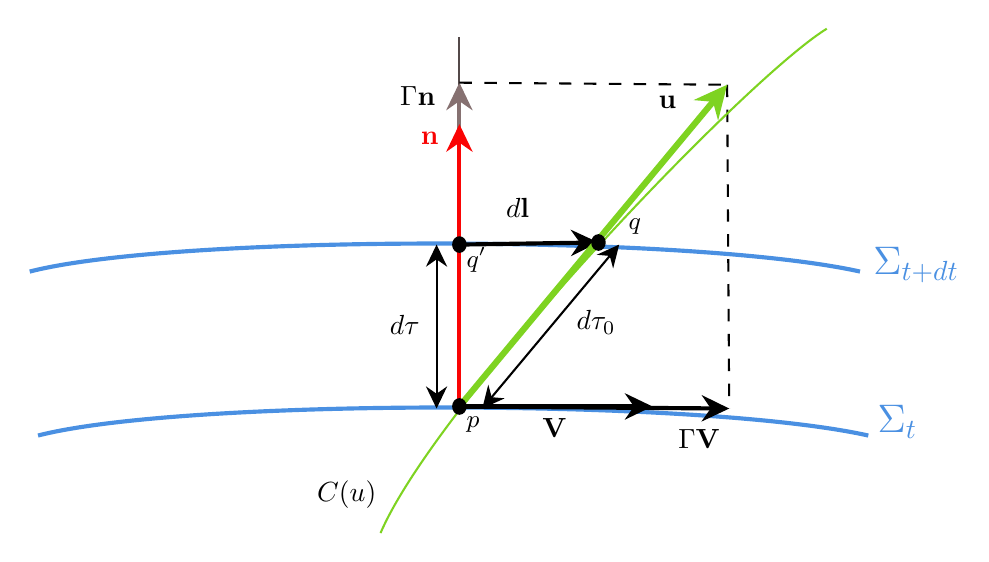
\begin{tikzpicture}[x=0.75pt,y=0.75pt,yscale=-1,xscale=1]
%uncomment if require: \path (0,300); %set diagram left start at 0, and has height of 300

%Curve Lines [id:da26959026957534016] 
\draw [color={rgb, 255:red, 74; green, 144; blue, 226 }  ,draw opacity=1 ][line width=1.5]    (140,123) .. controls (210,105) and (459,105) .. (540,123) ;
%Curve Lines [id:da07724871314422188] 
\draw [color={rgb, 255:red, 74; green, 144; blue, 226 }  ,draw opacity=1 ][line width=1.5]    (144,202) .. controls (214,184) and (463,184) .. (544,202) ;
%Straight Lines [id:da12146828542495947] 
\draw [color={rgb, 255:red, 83; green, 73; blue, 73 }  ,draw opacity=1 ]   (347,10) -- (347,188) ;
%Straight Lines [id:da4988789475788382] 
\draw [color={rgb, 255:red, 134; green, 113; blue, 113 }  ,draw opacity=1 ][line width=1.5]    (347,188) -- (347,36) ;
\draw [shift={(347,32)}, rotate = 90] [fill={rgb, 255:red, 134; green, 113; blue, 113 }  ,fill opacity=1 ][line width=0.08]  [draw opacity=0] (13.4,-6.43) -- (0,0) -- (13.4,6.44) -- (8.9,0) -- cycle    ;
%Straight Lines [id:da06082036119053047] 
\draw [color={rgb, 255:red, 250; green, 4; blue, 4 }  ,draw opacity=1 ][fill={rgb, 255:red, 255; green, 255; blue, 255 }  ,fill opacity=1 ][line width=1.5]    (347,188) -- (347,56) ;
\draw [shift={(347,52)}, rotate = 90] [fill={rgb, 255:red, 250; green, 4; blue, 4 }  ,fill opacity=1 ][line width=0.08]  [draw opacity=0] (13.4,-6.43) -- (0,0) -- (13.4,6.44) -- (8.9,0) -- cycle    ;
%Straight Lines [id:da4667101574604672] 
\draw [line width=1.5]    (347,110) -- (410,109.06) ;
\draw [shift={(414,109)}, rotate = 179.14] [fill={rgb, 255:red, 0; green, 0; blue, 0 }  ][line width=0.08]  [draw opacity=0] (13.4,-6.43) -- (0,0) -- (13.4,6.44) -- (8.9,0) -- cycle    ;
%Straight Lines [id:da1570235924345741] 
\draw  [dash pattern={on 4.5pt off 4.5pt}]  (347,32) -- (476,33) ;
%Straight Lines [id:da5125772773112368] 
\draw  [dash pattern={on 4.5pt off 4.5pt}]  (476,33) -- (477,189) ;
%Straight Lines [id:da8458059489889164] 
\draw [line width=1.5]    (347,188) -- (473,188.97) ;
\draw [shift={(477,189)}, rotate = 180.44] [fill={rgb, 255:red, 0; green, 0; blue, 0 }  ][line width=0.08]  [draw opacity=0] (13.4,-6.43) -- (0,0) -- (13.4,6.44) -- (8.9,0) -- cycle    ;
%Curve Lines [id:da5376288312211105] 
\draw [color={rgb, 255:red, 126; green, 211; blue, 33 }  ,draw opacity=1 ][line width=0.75]    (309,249) .. controls (336,186) and (485,30) .. (524,6) ;
%Straight Lines [id:da021439346537276638] 
\draw [color={rgb, 255:red, 126; green, 211; blue, 33 }  ,draw opacity=1 ][line width=2.25]    (347,188) -- (472.8,36.84) ;
\draw [shift={(476,33)}, rotate = 129.77] [fill={rgb, 255:red, 126; green, 211; blue, 33 }  ,fill opacity=1 ][line width=0.08]  [draw opacity=0] (16.07,-7.72) -- (0,0) -- (16.07,7.72) -- (10.67,0) -- cycle    ;
%Straight Lines [id:da2721548710880187] 
\draw [line width=1.5]    (347,188) -- (436,188) ;
\draw [shift={(440,188)}, rotate = 180] [fill={rgb, 255:red, 0; green, 0; blue, 0 }  ][line width=0.08]  [draw opacity=0] (13.4,-6.43) -- (0,0) -- (13.4,6.44) -- (8.9,0) -- cycle    ;
%Straight Lines [id:da9135435453405968] 
\draw    (336,113) -- (336,186) ;
\draw [shift={(336,189)}, rotate = 270] [fill={rgb, 255:red, 0; green, 0; blue, 0 }  ][line width=0.08]  [draw opacity=0] (10.72,-5.15) -- (0,0) -- (10.72,5.15) -- (7.12,0) -- cycle    ;
\draw [shift={(336,110)}, rotate = 90] [fill={rgb, 255:red, 0; green, 0; blue, 0 }  ][line width=0.08]  [draw opacity=0] (10.72,-5.15) -- (0,0) -- (10.72,5.15) -- (7.12,0) -- cycle    ;
%Straight Lines [id:da7439837710034684] 
\draw    (422.08,112.3) -- (359.92,186.7) ;
\draw [shift={(358,189)}, rotate = 309.88] [fill={rgb, 255:red, 0; green, 0; blue, 0 }  ][line width=0.08]  [draw opacity=0] (10.72,-5.15) -- (0,0) -- (10.72,5.15) -- (7.12,0) -- cycle    ;
\draw [shift={(424,110)}, rotate = 129.88] [fill={rgb, 255:red, 0; green, 0; blue, 0 }  ][line width=0.08]  [draw opacity=0] (10.72,-5.15) -- (0,0) -- (10.72,5.15) -- (7.12,0) -- cycle    ;
%Shape: Ellipse [id:dp6764690294244228] 
\draw  [fill={rgb, 255:red, 0; green, 0; blue, 0 }  ,fill opacity=1 ] (344,110) .. controls (344,108.07) and (345.34,106.5) .. (347,106.5) .. controls (348.66,106.5) and (350,108.07) .. (350,110) .. controls (350,111.93) and (348.66,113.5) .. (347,113.5) .. controls (345.34,113.5) and (344,111.93) .. (344,110) -- cycle ;
%Shape: Ellipse [id:dp4250053809271229] 
\draw  [fill={rgb, 255:red, 0; green, 0; blue, 0 }  ,fill opacity=1 ] (344,188) .. controls (344,186.07) and (345.34,184.5) .. (347,184.5) .. controls (348.66,184.5) and (350,186.07) .. (350,188) .. controls (350,189.93) and (348.66,191.5) .. (347,191.5) .. controls (345.34,191.5) and (344,189.93) .. (344,188) -- cycle ;
%Shape: Ellipse [id:dp9571825606449815] 
\draw  [fill={rgb, 255:red, 0; green, 0; blue, 0 }  ,fill opacity=1 ] (411,109) .. controls (411,107.07) and (412.34,105.5) .. (414,105.5) .. controls (415.66,105.5) and (417,107.07) .. (417,109) .. controls (417,110.93) and (415.66,112.5) .. (414,112.5) .. controls (412.34,112.5) and (411,110.93) .. (411,109) -- cycle ;

% Text Node
\draw (547,185.9) node [anchor=north west][inner sep=0.75pt]  [font=\Large,color={rgb, 255:red, 74; green, 144; blue, 226 }  ,opacity=1 ]  {$\Sigma _{t}$};
% Text Node
\draw (545,109.9) node [anchor=north west][inner sep=0.75pt]  [font=\Large,color={rgb, 255:red, 74; green, 144; blue, 226 }  ,opacity=1 ]  {$\Sigma _{t+dt}$};
% Text Node
\draw (327,54.4) node [anchor=north west][inner sep=0.75pt]  [color={rgb, 255:red, 248; green, 2; blue, 2 }  ,opacity=1 ]  {$\mathbf{n}$};
% Text Node
\draw (317,32.4) node [anchor=north west][inner sep=0.75pt]    {$\Gamma \mathbf{n}$};
% Text Node
\draw (368,86.4) node [anchor=north west][inner sep=0.75pt]    {$d\mathbf{l}$};
% Text Node
\draw (441.5,36.9) node [anchor=north west][inner sep=0.75pt]    {$\mathbf{u}$};
% Text Node
\draw (451,197.4) node [anchor=north west][inner sep=0.75pt]    {$\Gamma \mathbf{V}$};
% Text Node
\draw (385.5,192.4) node [anchor=north west][inner sep=0.75pt]    {$\mathbf{V}$};
% Text Node
\draw (312,142.4) node [anchor=north west][inner sep=0.75pt]    {$d\tau $};
% Text Node
\draw (402,140.4) node [anchor=north west][inner sep=0.75pt]    {$d\tau _{0}$};
% Text Node
\draw (277,222.4) node [anchor=north west][inner sep=0.75pt]    {$C( u)$};
% Text Node
\draw (349,191.4) node [anchor=north west][inner sep=0.75pt]  [font=\small]  {$p$};
% Text Node
\draw (349,109.9) node [anchor=north west][inner sep=0.75pt]  [font=\small]  {$q'$};
% Text Node
\draw (427,95.9) node [anchor=north west][inner sep=0.75pt]  [font=\small]  {$q$};


\end{tikzpicture}
    \end{center}
    \label{fig:eulerian_velocity}
\end{figure}

To determine this vector, let us first consider a fluid element at a point $p\in \Sigma_t$.
Let $\tau$ be the Eulerian observer's \footnote{The Eulerian observer is the observer where it's velocity is the unit timelike vector $\mathbf{n}$ in Fig.\ref{fig:foliation}} proper time at $p$.
After a coordinate time $t+dt$, the fluid element as moved to the point $q\in \Sigma_{t+dt}$. Locally the event $q'$, which for the observer happens at a time $\tau + d\tau$, is given by the orthogonal projection of $q$ onto the observer's worldline\footnote{The space of simultaneous events for the Eulerian observer is the space orthogonal to his 4-velocity $\mathbf{n}$.}.
Defining the infinitesimal distance between $q$ and $q'$ as $d\mathbf{l}$. Then $d\tau_0$ be the proper time increment of the fluid, this time is related with the proper time of the observer by the Lorentz factor, $\Gamma$,
\begin{equation}
    d\tau := \Gamma d\tau_0
    \label{eqn:time_dilation}
\end{equation}

We also get the triangle identity,
\begin{equation}
    d\tau_0 \mathbf{u} = d\tau \mathbf{n} + d\mathbf{l}
    \label{eqn:triangle_identity}
\end{equation}
by taking the scalar product with $\mathbf{n}$,
\begin{equation}
    d\tau_0 \mathbf{u} \cdot \mathbf{n} = d\tau \underbrace{\mathbf{n} \cdot \mathbf{n}}_{-1} + \underbrace{d\mathbf{l} \cdot \mathbf{n}}_{0}
\end{equation}
hence with the relation in Eq.(\ref{eqn:time_dilation}),
\begin{equation}
    \Gamma=-\mathbf{u} \cdot \mathbf{n}
\end{equation}
with respect to the coordinates $(t,x^i)$,
\begin{equation}
    \Gamma = Nu^0
\end{equation}

The fluid velocity relative to the Eulerian observer is defined as,
\begin{equation}
    \mathbf{V}=\frac{d\mathbf{l}}{d\tau}.
    \label{eqn:definition_eulerian_fluid_velocity}
\end{equation}

By dividing the identity \ref{eqn:triangle_identity} by $d\tau$ and using Eq.\ref{eqn:time_dilation},
\begin{equation}
    \mathbf{u}=\Gamma(\mathbf{n}+\mathbf{V}).
    \label{eqn:general_fluid_expression}
\end{equation}

We see that the fluid 4-velocity, $\mathbf{u}$, is now decomposed into a timelike and a spacelike part. The normalization of the fluid 4-velocity, $\mathbf{u}\cdot \mathbf{u}=-1$, gives us,
\begin{equation}
    \Gamma=(1-\mathbf{V}\cdot \mathbf{V})^{-1/2}.
    \label{eqn:general_gamma}
\end{equation} 

Notice this expression is similar to the Lorentz factor in special relativity, except the scalar product here is taken with the curved metric, instead of a flat metric.

Now it is worth to see how the Eulerian vector $\mathbf{V}$, is expressed in the base of coordinates $(t,x^i)$. 
The fluid coordinate velocity is defined by,
\begin{equation}
    \mathbf{v}:= \frac{d\mathbf{x}}{dt}
    \label{fig:definition_fluid_coordinate_velocity}
\end{equation}
where $d\mathbf{x}$ is the displacement between the fluid worline and the line of constant spatial coordinates.

\begin{figure}[h]
    \centering
    \begin{center}
\tikzset{every picture/.style={line width=0.75pt}} %set default line width to 0.75pt        

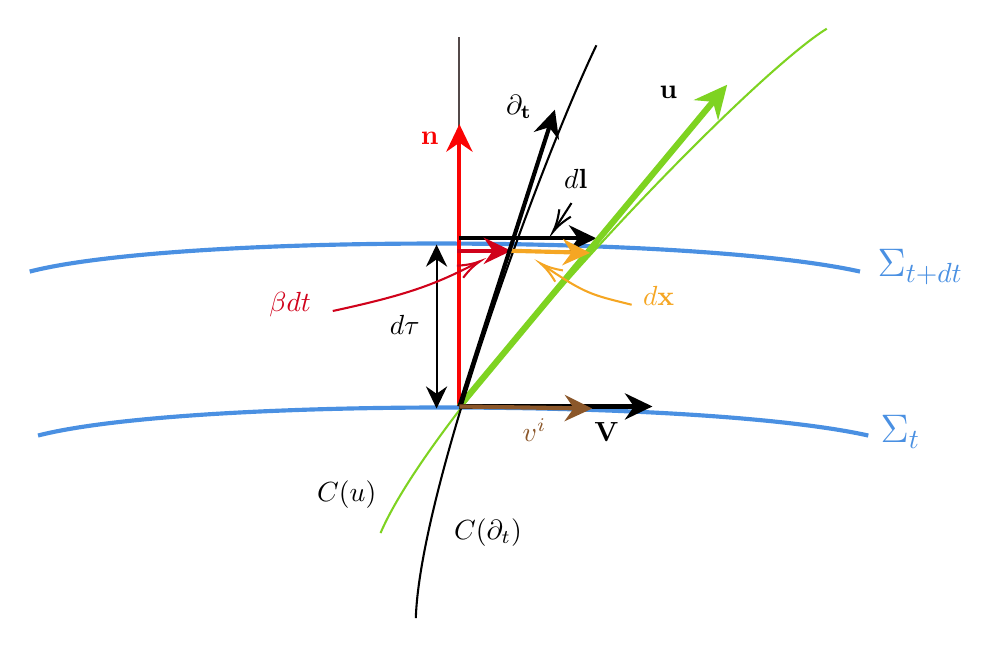
\begin{tikzpicture}[x=0.75pt,y=0.75pt,yscale=-1,xscale=1]
%uncomment if require: \path (0,300); %set diagram left start at 0, and has height of 300

%Curve Lines [id:da789582644087943] 
\draw [color={rgb, 255:red, 74; green, 144; blue, 226 }  ,draw opacity=1 ][line width=1.5]    (140,123) .. controls (210,105) and (459,105) .. (540,123) ;
%Curve Lines [id:da9861109193070141] 
\draw [color={rgb, 255:red, 74; green, 144; blue, 226 }  ,draw opacity=1 ][line width=1.5]    (144,202) .. controls (214,184) and (463,184) .. (544,202) ;
%Straight Lines [id:da924960238207858] 
\draw [color={rgb, 255:red, 83; green, 73; blue, 73 }  ,draw opacity=1 ]   (347,10) -- (347,188) ;
%Straight Lines [id:da8596667617367413] 
\draw [color={rgb, 255:red, 250; green, 4; blue, 4 }  ,draw opacity=1 ][fill={rgb, 255:red, 255; green, 255; blue, 255 }  ,fill opacity=1 ][line width=1.5]    (347,188) -- (347,56) ;
\draw [shift={(347,52)}, rotate = 90] [fill={rgb, 255:red, 250; green, 4; blue, 4 }  ,fill opacity=1 ][line width=0.08]  [draw opacity=0] (13.4,-6.43) -- (0,0) -- (13.4,6.44) -- (8.9,0) -- cycle    ;
%Straight Lines [id:da42329334891440695] 
\draw [line width=1.5]    (347,107) -- (409,107) ;
\draw [shift={(413,107)}, rotate = 180] [fill={rgb, 255:red, 0; green, 0; blue, 0 }  ][line width=0.08]  [draw opacity=0] (13.4,-6.43) -- (0,0) -- (13.4,6.44) -- (8.9,0) -- cycle    ;
%Curve Lines [id:da49959183381810357] 
\draw [color={rgb, 255:red, 126; green, 211; blue, 33 }  ,draw opacity=1 ][line width=0.75]    (309,249) .. controls (332.46,194.26) and (448.01,69.32) .. (503.5,21.75) .. controls (511.88,14.57) and (518.88,9.15) .. (524,6) ;
%Straight Lines [id:da7852131648516276] 
\draw [color={rgb, 255:red, 126; green, 211; blue, 33 }  ,draw opacity=1 ][line width=2.25]    (347,188) -- (472.8,36.84) ;
\draw [shift={(476,33)}, rotate = 129.77] [fill={rgb, 255:red, 126; green, 211; blue, 33 }  ,fill opacity=1 ][line width=0.08]  [draw opacity=0] (16.07,-7.72) -- (0,0) -- (16.07,7.72) -- (10.67,0) -- cycle    ;
%Straight Lines [id:da33165143523679497] 
\draw [line width=1.5]    (347,188) -- (436,188) ;
\draw [shift={(440,188)}, rotate = 180] [fill={rgb, 255:red, 0; green, 0; blue, 0 }  ][line width=0.08]  [draw opacity=0] (13.4,-6.43) -- (0,0) -- (13.4,6.44) -- (8.9,0) -- cycle    ;
%Straight Lines [id:da38801371990156497] 
\draw    (336,113) -- (336,186) ;
\draw [shift={(336,189)}, rotate = 270] [fill={rgb, 255:red, 0; green, 0; blue, 0 }  ][line width=0.08]  [draw opacity=0] (10.72,-5.15) -- (0,0) -- (10.72,5.15) -- (7.12,0) -- cycle    ;
\draw [shift={(336,110)}, rotate = 90] [fill={rgb, 255:red, 0; green, 0; blue, 0 }  ][line width=0.08]  [draw opacity=0] (10.72,-5.15) -- (0,0) -- (10.72,5.15) -- (7.12,0) -- cycle    ;
%Curve Lines [id:da47910404253123684] 
\draw [color={rgb, 255:red, 0; green, 0; blue, 0 }  ,draw opacity=1 ][line width=0.75]    (326,290) .. controls (328,228) and (387,68) .. (413,14) ;
%Straight Lines [id:da9696842560642254] 
\draw [color={rgb, 255:red, 208; green, 2; blue, 27 }  ,draw opacity=1 ][line width=1.5]    (346,113) -- (368,113) ;
\draw [shift={(372,113)}, rotate = 180] [fill={rgb, 255:red, 208; green, 2; blue, 27 }  ,fill opacity=1 ][line width=0.08]  [draw opacity=0] (13.4,-6.43) -- (0,0) -- (13.4,6.44) -- (8.9,0) -- cycle    ;
%Straight Lines [id:da025515408244085935] 
\draw [color={rgb, 255:red, 245; green, 166; blue, 35 }  ,draw opacity=1 ][line width=1.5]    (372,113) -- (406,113.89) ;
\draw [shift={(410,114)}, rotate = 181.51] [fill={rgb, 255:red, 245; green, 166; blue, 35 }  ,fill opacity=1 ][line width=0.08]  [draw opacity=0] (13.4,-6.43) -- (0,0) -- (13.4,6.44) -- (8.9,0) -- cycle    ;
%Straight Lines [id:da11283948545816691] 
\draw [line width=1.5]    (347,188) -- (391.78,48.81) ;
\draw [shift={(393,45)}, rotate = 107.83] [fill={rgb, 255:red, 0; green, 0; blue, 0 }  ][line width=0.08]  [draw opacity=0] (13.4,-6.43) -- (0,0) -- (13.4,6.44) -- (8.9,0) -- cycle    ;
%Curve Lines [id:da7075013819427496] 
\draw [color={rgb, 255:red, 208; green, 2; blue, 27 }  ,draw opacity=1 ]   (286,142) .. controls (322.08,134.2) and (335.34,129.25) .. (355.44,118.81) ;
\draw [shift={(357,118)}, rotate = 152.35] [color={rgb, 255:red, 208; green, 2; blue, 27 }  ,draw opacity=1 ][line width=0.75]    (10.93,-3.29) .. controls (6.95,-1.4) and (3.31,-0.3) .. (0,0) .. controls (3.31,0.3) and (6.95,1.4) .. (10.93,3.29)   ;
%Curve Lines [id:da6564312272230666] 
\draw [color={rgb, 255:red, 245; green, 166; blue, 35 }  ,draw opacity=1 ]   (430,139) .. controls (410.5,134.13) and (408.11,134) .. (387.61,120.1) ;
\draw [shift={(386,119)}, rotate = 34.29] [color={rgb, 255:red, 245; green, 166; blue, 35 }  ,draw opacity=1 ][line width=0.75]    (10.93,-3.29) .. controls (6.95,-1.4) and (3.31,-0.3) .. (0,0) .. controls (3.31,0.3) and (6.95,1.4) .. (10.93,3.29)   ;
%Straight Lines [id:da08103496135612642] 
\draw    (401,90) -- (393.08,102.32) ;
\draw [shift={(392,104)}, rotate = 302.74] [color={rgb, 255:red, 0; green, 0; blue, 0 }  ][line width=0.75]    (10.93,-3.29) .. controls (6.95,-1.4) and (3.31,-0.3) .. (0,0) .. controls (3.31,0.3) and (6.95,1.4) .. (10.93,3.29)   ;
%Straight Lines [id:da05971548333425181] 
\draw [color={rgb, 255:red, 139; green, 87; blue, 42 }  ,draw opacity=1 ][line width=1.5]    (347,188) -- (407,188.94) ;
\draw [shift={(411,189)}, rotate = 180.9] [fill={rgb, 255:red, 139; green, 87; blue, 42 }  ,fill opacity=1 ][line width=0.08]  [draw opacity=0] (13.4,-6.43) -- (0,0) -- (13.4,6.44) -- (8.9,0) -- cycle    ;

% Text Node
\draw (548.5,190.9) node [anchor=north west][inner sep=0.75pt]  [font=\Large,color={rgb, 255:red, 74; green, 144; blue, 226 }  ,opacity=1 ]  {$\Sigma _{t}$};
% Text Node
\draw (547,110.9) node [anchor=north west][inner sep=0.75pt]  [font=\Large,color={rgb, 255:red, 74; green, 144; blue, 226 }  ,opacity=1 ]  {$\Sigma _{t+dt}$};
% Text Node
\draw (327,54.4) node [anchor=north west][inner sep=0.75pt]  [color={rgb, 255:red, 248; green, 2; blue, 2 }  ,opacity=1 ]  {$\mathbf{n}$};
% Text Node
\draw (396,72.4) node [anchor=north west][inner sep=0.75pt]    {$d\mathbf{l}$};
% Text Node
\draw (442,32.4) node [anchor=north west][inner sep=0.75pt]    {$\mathbf{u}$};
% Text Node
\draw (410.5,194.4) node [anchor=north west][inner sep=0.75pt]    {$\mathbf{V}$};
% Text Node
\draw (312,142.4) node [anchor=north west][inner sep=0.75pt]    {$d\tau $};
% Text Node
\draw (277,222.4) node [anchor=north west][inner sep=0.75pt]    {$C( u)$};
% Text Node
\draw (343,240.4) node [anchor=north west][inner sep=0.75pt]    {$C( \partial _{t})$};
% Text Node
\draw (368,36.4) node [anchor=north west][inner sep=0.75pt]    {$\mathbf{\partial _{t}}$};
% Text Node
\draw (254,131.4) node [anchor=north west][inner sep=0.75pt]  [color={rgb, 255:red, 208; green, 2; blue, 27 }  ,opacity=1 ]  {$\mathbf{\beta } dt$};
% Text Node
\draw (434,128.4) node [anchor=north west][inner sep=0.75pt]  [color={rgb, 255:red, 245; green, 166; blue, 35 }  ,opacity=1 ]  {$d\mathbf{x}$};
% Text Node
\draw (376,192.4) node [anchor=north west][inner sep=0.75pt]  [color={rgb, 255:red, 139; green, 87; blue, 42 }  ,opacity=1 ]  {$v^{i}$};


\end{tikzpicture}
    \end{center}
    \label{fig:eulerian_velocity}
\end{figure}

From the definition of the shift vector, and with the help of the Fig.\ref{fig:eulerian_velocity},
\begin{equation}
    d\mathbf{l} = \bm{\beta} dt + d\mathbf{x}
\end{equation}
dividing this relation with $d\tau$, using Eqs.(\ref{eqn:definition_eulerian_fluid_velocity}) and (\ref{fig:definition_fluid_coordinate_velocity}),
\begin{equation}
    \mathbf{V}=\frac{1}{N}(\bm{\beta}+\mathbf{v}).
    \label{eqn:eulerian_fluid_velocity_expression}
\end{equation}

Where the components of $u_\mu$ and $u^\mu$ are \cite{Buchert_2020},
\begin{equation}
    u_\mu = \frac{\Gamma}{N}(-N^2+\beta^k(\beta_k+v_k),\beta_i+v_i), \qquad u^\mu = \frac{\Gamma}{N}(1,v^i)
    \label{eqn:upper_lower_fluid}
\end{equation}
check the footnote for more detail on how to obtain $u_\mu$\footnote{Let $\bm{\chi}$ be a spatial vector, $\chi^0=0$ (however $\chi_0\neq 0$) and it must satisfy, $n^\alpha \chi_\alpha=0$, which in turn gives us that $\chi_0=\beta^i\chi_i$.}.


\subsection{Decomposition of the covariant derivative of the four-velocity}

The operator that projects tensors onto the local rest frames of the fluid is, $\mathbf{b}=b_{\mu\nu}dx^\mu \otimes dx^\nu$,
\begin{equation}
    b_{\mu\nu}:=g_{\mu\nu}+u_\mu u_\nu,\qquad b_{\alpha\mu}u^\alpha=0,\qquad b^\mu_\alpha b^\alpha_\nu = b^\mu_\nu,\qquad b^{\alpha\beta}b_{\alpha\beta}=3.
\end{equation}
The projectors $\mathbf{b}$ and $\mathbf{h}$ mainly differ due to the tilt between $\mathbf{u}$ and $\mathbf{n}$.
Projected quantities using $\mathbf{b}$ or $\mathbf{h}$, represent what observers moving with $\mathbf{u}$ or $\mathbf{n}$ measure, respectively.


\subsection{Decomposition of the energy-momentum tensor}
The most important factor behind the usage of these two vectors, namely the Eulerian's and the fluid's velocities, $\mathbf{n}$ and $\mathbf{u}$, respectively, is their role in the interpretation of the energy-momentum tensor.

The decomposition with respect to the rest fluid is,
\begin{equation}
    T_{\mu\nu}=\rho u_\mu u_\nu + 2q_{(\mu}u_{\nu)} + \pi_{\mu\nu} + P b_{\mu\nu},
    \label{eqn:general_decomposition_energy_tensor_fluid}
\end{equation}
where $\rho$ is the energy density, $q_\mu$ is the spatial heat vector, $\pi_{\mu\nu}$ is the spatial and traceless anisotropic pressure, and $P$ is the isotropic pressure, all w.r.t the fluid's rest frames.

The decomposition with respect to the Normal frames,
\begin{equation}
    T_{\mu\nu} = E n_\mu n_\nu + 2J_{(\mu}n_{\nu)}+ S_{\mu\nu},
    \label{eqn:general_decomposition_energy_tensor_normal}
\end{equation}
where $E$ is the energy density of the fluid, $J_\mu$ is the momentum density, and $S_{\mu\nu}$ is the stress density, all w.r.t the normal vector.

Now we want to see the relation between $E$ and $\rho$, so that later we can substitute it in the Friedmann equation.

The energy density,
\begin{equation}
    E=\Gamma^2 \rho + (\Gamma^2-1)P+2\Gamma v^\alpha q_\alpha + V^\alpha V^\beta \pi_{\alpha\beta}
    \label{eqn:general_energy_fluid_normal}
\end{equation}

The pressure,
\begin{equation}
    S=(\Gamma^2-1)\rho + (\Gamma^2+2)P+2\Gamma V^\alpha q_\alpha + V^\alpha V^\beta \pi_{\alpha\beta}
    \label{eqn:general_shear_fluid_normal}
\end{equation}




\section{Time derivatives}


We have presented in Fig.\eqref{fig:foliation}, three different congruences and therefore multiple time derivatives can arise \cite{Buchert_2020}:
\begin{itemize}
    \item Comoving derivative along the normal flow and according to the proper time $\tau$, i.e. $d/d\tau$.
    \item Comoving derivative along the fluid flow and according to the proper time $\tau_0$, i.e. $d/d\tau_0$.
    \item Comoving derivative along the normal flow and according to the coordinate time, i.e. $d/dt$.
    \item Comoving derivative along the fluid flow and according to the coordinate time, i.e. $D/Dt$.
    \item Partial coordinate time derivative along the curves of $x^i=\text{const.}$, i.e. $\partial/\partial t:=\partial_t|_{x^i}$ .
\end{itemize}

Let $\mathbf{F}$ be a tensor of arbitrary rank. We can relate the $d/dt$ and $\partial_t|_{x^i}$ by,
\begin{equation}
    \frac{d\mathbf{F}}{dt}=\left.\frac{\partial \mathbf{F}}{\partial t}\right|_{X^i}=\left.\frac{\partial \mathbf{F}}{\partial t}\right|_{x^i}+\left.\frac{\partial x^i}{\partial t}\right|_{X^i}\frac{\partial \mathbf{F}}{\partial x^i}=\left.\frac{\partial \mathbf{F}}{\partial t}\right|_{x^i}-\beta^i\frac{\partial \mathbf{F}}{\partial x^i},
    \label{eqn:normal_total_time_expression}
\end{equation}
where $X^i$ are the comoving spatial coordinates w.r.t the normal flow. From the \cref{eqn:def_normal_vector_upper} we obtain.
\begin{equation}
    n^\mu\partial_\mu \mathbf{F}=\frac{d\mathbf{F}}{d\tau}=\frac{1}{N}\frac{d\mathbf{F}}{dt}.
    \label{eqn:relation_total_time_normal_vec}
\end{equation}

The fluid's time derivative, can relate the $D/Dt$ and $\partial_t|_{x^i}$ by,
\begin{equation}
    \frac{D\mathbf{F}}{Dt}=\left.\frac{\partial \mathbf{F}}{\partial t}\right|_{X^i}=\left.\frac{\partial \mathbf{F}}{\partial t}\right|_{x^i}+\left.\frac{\partial x^i}{\partial t}\right|_{X^i}\frac{\partial \mathbf{F}}{\partial x^i}=\left.\frac{\partial \mathbf{F}}{\partial t}\right|_{x^i}-\beta^i\frac{\partial \mathbf{F}}{\partial x^i},
    \label{eqn:fluid_total_time_expression}
\end{equation}
where now $X^i$ are the comoving spatial coordinates w.r.t the fluid flow. From the \cref{eqn:upper_lower_fluid} we obtain.
\begin{equation}
    u^\mu\partial_\mu \mathbf{F}=\frac{d\mathbf{F}}{d\tau_0}=\frac{\Gamma}{N}\frac{D\mathbf{F}}{Dt}.
    \label{eqn:relation_total_time_fluid_vec}
\end{equation}



\section{Kinematical quantities}

In the 3+1 formalism, it is useful to introduce the spatial connection $\mathbf{D}$, i.e. the three-covariant derivative associated with the metric $\mathbf{h}$, is defined as
\begin{equation}
    D_\mu T^{\alpha_1\cdots\alpha_p}{}_{\beta_1\cdots\beta_q}=h^{\alpha_1}_{\gamma_1}\cdots h^{\alpha_p}_{\gamma_p}h^{\delta_1}_{\beta_1}\cdots h^{\delta_q}_{\beta_q} h_\mu^\nu \nabla_\nu T^{\gamma_1\cdots\gamma_p}{}_{\delta_1\cdots\delta_q},
    \label{eqn:spatial_cov_dev_def}
\end{equation}
where $\nabla$ is the four-covariant derivative. Here the spatial connection satisfies the metric compatability,
\begin{equation}
    D_\mu h_{\alpha\beta}=0.
\end{equation}

The Frobenius theorem in \cref{app:frobenius} states that a foliation orthogonal to the fluid is only possible when there is no vorticity, and furthermore we will see that the three-torsion is proportional to vorticity (in the observers frame).
Therefore this connection has to be torsion-free, and a Levi-Civita connection. 
Notice that here we construct the connection around the observer, by using $\mathbf{h}$, if we were to use the fluid we would obtain a connection with metric compatability but under the presence of torsion. 

The acceleration vector is given by
\begin{equation}
    A_\alpha:=n^\mu \nabla_\mu n_\alpha=D_\alpha\ln N,
    \label{eqn:acceleration_normal}
\end{equation}
where in the last equality we used \cref{eqn:def_normal_vector_upper,eqn:def_normal_vector_lower}. 
Here it is noticable that if $N=1$ we describe a geodesic observer.

One can decompose the four-velocity of the normal vector using \cref{eqn:spatial_cov_dev_def}
\begin{equation}
    \nabla_\beta n_\alpha = g_\beta^\mu \nabla_\mu n_\alpha = (h_\beta^\mu-n_\beta n^\mu)\nabla_\mu n_\alpha=-n_\beta A_\alpha + D_\beta n_\alpha,
\end{equation}
where the last term is the extrinsic curvature, given by
\begin{equation}
    K_{\alpha\beta}:=D_\beta n_\alpha. 
\end{equation}

The extrinsic curvature is a type of curvature in hypersurfaces, that defines the bending of the hypersurface domain $\Sigma$ in the spacetime manifold $\mathcal{M}$.
It can be decomposed into a traceful and traceless part by
\begin{equation}
    K_{\alpha\beta}=\frac{1}{3}Kh_{\alpha\beta}+A_{\alpha\beta},
\end{equation}
where $K$ and $A_{\alpha\beta}$ are, respectively, the rate of expansion and shear viewed from the observer's perspective.
If a tensor field is perpendicular to the normal vector, e.g. $n^\nu K_{\mu\nu}=0$, then all its independent information lies in $K_{ij}$, which is the usual form we encounter in literature.


In the fluid's perspective the extrinsic curvature is
\begin{equation}
    \Theta_{\alpha\beta}:=D^{(\mathbf{u})}_\beta u_\alpha=\frac{1}{3}\Theta b_{\alpha\beta} + \sigma_{\alpha\beta} + w_{\alpha\beta},
\end{equation}
where $\Theta$, $\sigma_{\alpha\beta}$ and $w_{\alpha\beta}$ are the rate of expansion, shear and vorticity of the fluid.

From the spatial connection introduced, we also obtain a new type of curvature, the intrinsic curvature $\prescript{3}{}{\mathbf{R}}$.
The intrinsic curvature measures the non-commutativity between two consecutive three-covariant derivates $\mathbf{D}$, by the Ricci identity:
\begin{equation}
    \left[D_i,D_j\right]v^k=\prescript{3}{}R^{k}{}_{lij}v^l,
    \label{eqn:spatial_ricci_identity}
\end{equation}
where $\mathbf{v}$ is a spatial vector and the prescript 3 indicates explicitely the quantity is spatial. 
When building the formalism using the fluid flow, it would yield an additional term proportional to a non-zero torsion $\prescript{3}{}{\mathbf{T}}$.%+h^k_m \prescript{3}{}T^{l}{}_{ij}\nabla_l v^m


\section{Gauss-Codazzi-Ricci Relations}

In this section we will introduce the decompositions of the spacetime Riemann tensor derived in \cref{app:gauss,app:codazzi,app:ricci}.
These decompositions are in terms of the quantities in the previous section, namely the Riemann tensor associated with the metric $\mathbf{h}$, $\prescript{3}{}{\mathbf{R}}$, the extrinsic curvature $\mathbf{K}$, and the acceleration vector $\mathbf{A}$.

Throughout these relations we will not consider the extrinsic curvature symmetric. 
This choice is made so we can easily relate to the relations obtained using the fluid flow, where the vortivity is generally non-zero.

From the Codazzi relation in \cref{app:codazzi},
\begin{align}
    &\perp_u (R^\alpha{}_{\beta\gamma\delta} n^\beta)= h^\alpha_\epsilon h^\phi_\gamma h^\mu_\delta R^\epsilon{}_{\beta\phi\mu} u^\beta= 4 K_{[\alpha\delta]}A^\alpha + D_\gamma K^\alpha{}_\delta - D_\delta K^\alpha{}_\gamma \Leftrightarrow \times \delta_\gamma^\alpha\\
    &\Leftrightarrow h^\phi_\epsilon h^\mu_\delta R^\epsilon{}_{\beta\phi\mu} n^\beta = 4 K_{[\alpha\delta]}A^\alpha + D_\alpha K^\alpha{}_\delta - D_\delta K^\alpha{}_\alpha \Leftrightarrow \\
    &\Leftrightarrow (\delta^\phi_\epsilon + n^\phi n_\epsilon)h^\mu_\delta R^\epsilon{}_{\beta\phi\mu} n^\beta = 4 K_{[\alpha\delta]}A^\alpha + D_\alpha K^\alpha{}_\delta - D_\delta K \Leftrightarrow \\
    &\Leftrightarrow \delta^\phi_\epsilon h^\mu_\delta R^\epsilon{}_{\beta\phi\mu} n^\beta  + h^\mu_\delta R^\epsilon{}_{\beta\phi\mu} n^\beta  n^\phi n_\epsilon = 4 K_{[\alpha\delta]}A^\alpha + D_\alpha K^\alpha{}_\delta - D_\delta K\Leftrightarrow \\
    &\Leftrightarrow  h^\mu_\delta R^\epsilon{}_{\beta\epsilon\mu} n^\beta  + h^\mu_\delta \underbrace{R_{\epsilon\beta\phi\mu}}_{\beta \leftrightarrow \epsilon \text{ Anti-symmetric}}   n^\phi \underbrace{n^\beta n^\epsilon}_{\text{Symmetric}} = 4 \Theta_{[\alpha\delta]}A^\alpha + D_\alpha K^\alpha{}_\delta - D_\delta K \Leftrightarrow \\
    &\Leftrightarrow h^\mu_\delta R_{\beta\mu} n^\beta = 4 K_{[\alpha\delta]}A^\alpha + D_\alpha K^\alpha{}_\delta - D_\delta K
    \label{eqn:ricci_extradig_proj}
\end{align}

In \cref{app:gauss} we obtained
\begin{align}
    \perp_{\mathbf{n}} R^\alpha{}_{\beta\gamma\delta} = \prescript{3}{}R^\alpha{}_{\beta\gamma\delta}+K^\alpha{}_\gamma K_{\beta\delta}-K^\alpha{}_\delta K_{\beta\gamma}.
\end{align}

Contracting the $\alpha$ and $\gamma$ indices in the Gauss relation, we obtain
\begin{align}
    \perp_{\mathbf{n}} R_{\alpha\delta}  = \prescript{3}{}R_{\alpha\delta}+KK_{\alpha\delta}-K^\gamma{}_\delta K_{\alpha\gamma} - h^\beta_\alpha h^\mu_\delta R_{\epsilon\beta\phi\mu} n^\phi n^\epsilon,
    \label{eqn:gauss_relation_proj}
\end{align}
where the last term, we want the $\phi$ and $\epsilon$ to be the second and last indices of the Riemann tensor and using the Ricci relation in \cref{app:ricci}
\begin{align}
    h^\beta_\alpha h^\mu_\delta R_{\epsilon\beta\phi\mu} n^\phi n^\epsilon= h_{\beta\alpha} h^\mu_\delta R^\beta{}_{\epsilon\mu\phi} n^\phi n^\epsilon = \perp_u(R_{\alpha\epsilon\delta\phi} n^\phi n^\epsilon) = D_\delta A_\alpha + A_\alpha A_\delta + K^\beta{}_\delta K_{\beta\alpha} - \dot{K}_{\alpha\delta},
    \label{eqn:ricci_relation}
\end{align}
where we define the overdot as $\dot{\mathbf{T}}=\mathcal{L}_{\mathbf{n}}\mathbf{T}$.

Inserting \cref{eqn:ricci_relation} in \cref{eqn:gauss_relation_proj}
\begin{align}
    \perp_{\mathbf{n}} R_{\alpha\delta}=\prescript{3}{}R_{\alpha\delta}+K K_{\alpha\delta}- D_\delta A_\alpha - A_\alpha A_\delta + \dot{K}_{\alpha\delta} -K^\beta{}_\delta (K_{\alpha\beta}+K_{\beta\alpha}).
    \label{eqn:ricci_spatial_proj}
\end{align}


From the Ricci relation in \cref{app:ricci},
\begin{align}
    &\perp_{\mathbf{n}} (R^\alpha{}_{\beta\gamma\delta} n^\beta n^\delta) = D_\gamma A^\alpha + A^\alpha A_\gamma + K^\delta{}_\gamma K_\delta{}^\alpha - \dot{K}^\alpha{}_\gamma \Leftrightarrow \times \delta^\gamma_\alpha\\
    &\Leftrightarrow  R_{\beta\delta}n^\beta n^\delta = D_\alpha A^\alpha + A^\alpha A_\alpha - K^\delta{}_\alpha K_\alpha{}^\delta -\dot{K}.
    \label{eqn:ricci_time_proj}
\end{align}


Contracting the indices in \cref{eqn:ricci_spatial_proj} and using \cref{eqn:ricci_time_proj}, we get the Ricci scalar decomposition:
\begin{align}
    R = \prescript{3}{}R+K^2 - 2(D^\alpha A_\alpha +  A_\alpha A^\alpha) + 2\dot{K}-K_{\alpha\beta}\dot{h}^{\alpha\beta}-K^{\alpha\beta}K_{\alpha\beta}.
    \label{eqn:ricci_scalar_decomp}
\end{align}





\section{Dynamical Equations}


From another definition of the extrinsic curvature with no vorticity:
\begin{align}
    K_{ij} := \frac{1}{2} \mathcal{L}_{\mathbf{n}} h_{ij},
\end{align}
i.e. the symmetric part of the extrinsic curvature. It is worth to note that $\mathcal{L}_{\mathbf{n}} h^{ij} \neq K^{ij}$ due to the Lie derivative's properties, in the \cref{app:formalism}. 
From this we can get the evolution equation for the metric $\mathbf{h}$:
\begin{equation}
    \frac{d h_{ij}}{dt} = 2NK_{ij}+(NV^k) \partial_k h_{ij} + h_{ik}\partial_j \beta^k + h_{kj}\partial_i \beta^k
\end{equation}


Considering a spacetime that obeys the Einstein equation:
\begin{equation}
    \mathbf{R}-\frac{1}{2}R\mathbf{g}=\kappa^2 \mathbf{T},
    \label{eqn:einstein_formalism}
\end{equation}
where $\kappa^2=8\pi G$. It can also be written as
\begin{equation}
    \mathbf{R}=\kappa^2 \left(\mathbf{T}-\frac{1}{2}T\mathbf{g}\right),
    \label{eqn:einstein_equiv}
\end{equation}
where $T$ is trace of the EM tensor.

We can project these equations in three ways: a full projection along the normal vector (and perpendicular to $\Sigma$); a mixed projection along the normal vector and the hypersurface; and a full projection onto $\Sigma$.

Projecting the \cref{eqn:einstein_formalism} along the normal vector in
\begin{equation}
    n^\mu n^\nu R_{\mu\nu}+\frac{1}{2}R=\kappa^2 T_{\mu\nu}n^\mu n^\nu,
\end{equation}
by using \cref{eqn:ricci_time_proj,eqn:ricci_scalar_decomp,eqn:general_decomposition_energy_tensor_normal}, we obtain the energy equation or called Hamiltonian constraint \cite{Gourgoulhon:2012ffd}:
\begin{equation}
    \frac{1}{2}\left(\prescript{3}{}R+K^2-K_{\mu\nu}K^{\mu\nu}\right)=\kappa^2 E,
    \label{eqn:energy_equation_normal}
\end{equation}
the equivalent equation for the fluid flow is
\begin{equation}
    \frac{1}{2}\left(\prescript{3}{}R_{(\mathbf{u})}+\Theta^2-\Theta_{\mu\nu}\Theta^{\nu\mu}\right)=\kappa^2\rho,
\end{equation}
where we stress the order of the indices in the last term inside the curved brackets.

Projecting \cref{eqn:einstein_formalism} along the normal vector and the hypersurface:
\begin{equation}
    h^\mu_\alpha n^\nu R_{\mu\nu}=\kappa^2 T_{\mu\nu} h^\mu_\alpha n^\nu
\end{equation}
by using \cref{eqn:ricci_extradig_proj,eqn:general_decomposition_energy_tensor_normal} we get the momentum constraint:
\begin{equation}
    D_i K - D_j K^j{}_i =\kappa^2 J_i,
\end{equation}
where we use spatial indeces as the equation only involves spatial quantities. For the fluid flow is
\begin{equation}
    D^{(\mathbf{u})}_\alpha \Theta - D^{(\mathbf{u})}_\beta \Theta^\beta{}_\alpha + 2w_{\alpha\beta}A^\beta_{(\mathbf{u})} =\kappa^2 q_\alpha.
    \label{eqn:momentum_equation_normal}
\end{equation}
 

Projecting \cref{eqn:einstein_equiv} onto the hypersurface
\begin{equation}
    \perp_{\mathbf{n}}R_{\mu\nu}=\kappa^2\perp_{\mathbf{n}}\left(T_{\mu\nu}-\frac{1}{2}T g_{\mu\nu}\right),
\end{equation}
by using \cref{eqn:ricci_spatial_proj,eqn:general_decomposition_energy_tensor_normal} we get
\begin{equation}
    \mathcal{L}_{\mathbf{n}}K_{\mu\nu}=\kappa^2\left(S_{\mu\nu}-\frac{1}{2}(S-E)h_{\mu\nu}\right)+N^{-1}D_\nu D_\mu N + K^\alpha{}_\nu(K_{\mu\alpha}+K_{\alpha\mu}) - KK_{\mu\nu}-\prescript{3}{}R_{\mu\nu},
    \nonumber
\end{equation}
notice again the above equation only contains spatial tensor fields, and therefore we can write with spatial indices:
\begin{equation}
    \mathcal{L}_{\mathbf{n}}K_{ij}=\kappa^2\left(S_{ij}-\frac{1}{2}(S-E)h_{ij}\right)+N^{-1}D_j D_i N + K^k{}_j(K_{i k}+K_{k i}) - KK_{ij}-\prescript{3}{}R_{ij},
\end{equation}
where we use \cref{eqn:acceleration_normal} to simplify $D_jA_i+A_jA_i=N^{-1}D_j D_i N$.

Instead of projecting the equivalent form of the Einstein equation, let us project the Einstein equation onto the hypersurface:
\begin{equation}
    \perp_{\mathbf{n}}R_{\mu\nu}-\frac{3}{2}R=\kappa^2  \perp_{\mathbf{n}} T_{\mu\nu},
\end{equation}
where taking the trace and using \cref{eqn:ricci_spatial_proj,eqn:general_decomposition_energy_tensor_normal} yields
\begin{align}
    &\prescript{3}{}R+K^2- N^{-1}D^i D_i N + h^{ij}\dot{K}_{ij}-K^{ij}K_{ji}-K^{ij}K_{ij}\\
    &\quad\quad- \frac{3}{2}\left(\prescript{3}{}R+K^2-  2N^{-1}D^i D_i N + 2\dot{K}-K_{ij}\dot{h}^{ij}-K^{ij}K_{ij}\right)=\kappa^2 S\Leftrightarrow\\
    &\Leftrightarrow \frac{1}{2}\left(-\prescript{3}{}R-K^2+ 4N^{-1}D^i D_i N -4 \dot{K}-3K_{ij}K^{ji}\right)=\kappa^2 S.
    \label{eqn:pressure_equation_normal}
\end{align}

From the conservation law $\nabla_\alpha T^{\alpha\beta}=0$, projecting along the fluid flow:
\begin{align}
    u_\beta\nabla_\alpha T^{\alpha\beta}=0&\Leftrightarrow u_\beta\nabla_\alpha\left(\rho u^\alpha u^\beta + 2q^{(\alpha} u^{\beta)} +\pi_{\alpha\beta} + P b_{\alpha\beta}\right)=0\Leftrightarrow \nonumber\\
    &\Leftrightarrow \frac{\Gamma}{N}\frac{D\rho}{Dt} + \Theta(\rho+P)=  - 2A^{(\mathbf{u})}_\alpha q^\alpha - D^{(\mathbf{u})}_\alpha q^\alpha -\pi^{\alpha\beta}\Sigma_{\alpha\beta}
    \label{eqn:energy_conserv_law_fluid},
\end{align}
where we use the total time derivative according to the fluid flow in \cref{eqn:relation_total_time_fluid_vec}.
And the energy conservation law according to the observer is
\begin{align}
    n_\beta\nabla_\alpha T^{\alpha\beta}=0&\Leftrightarrow n_\beta\nabla_\alpha\left(E n^\alpha n^\beta + 2J^{(\alpha} n^{\beta)} +S_{\alpha\beta}\right)=0\Leftrightarrow \nonumber\\
    &\Leftrightarrow\frac{1}{N}\frac{dE}{dt} + K\left(E+\frac{S}{3}\right)=  - 2A_\alpha J^\alpha - D_\alpha J^\alpha -S_{\alpha\beta}A^{\alpha\beta}.
    \label{eqn:energy_conserv_law_normal}
\end{align}

\section{Conformal 3+1 Formalism}

A conformal transformation is a mathematical operation that alters the spacetime metric while preserving angles but not distances, it is a very useful tool in modified theories as we will establish later, however for the moment let us focus in its role in the 3+1 formalism.

\subsection{Introduction}

A conformal transformation is given by
\begin{equation}
    g_{\mu\nu}\rightarrow \Tilde{g}_{\mu\nu}=\Omega^{-2}g_{\mu\nu}, \qquad g^{\mu\nu}\rightarrow \Tilde{g}^{\mu\nu}=\Omega^{2}g^{\mu\nu}
    \label{eqn:def_conf_transf}
\end{equation}
where $\Omega$ is some strictly positive scalar field. It is important to overstate that this transformation does not alter the basis of coordinates. 

Since the conformal metric is still a valid metric, there exists a unique Levi-Civita connection $\Tilde{\nabla}$ associated with it. Therefore, given a tensor field $\mathbf{T}$ with rank $\begin{pmatrix}p\\q\end{pmatrix}$, the covariant derivatives are related by
\begin{equation}
    \nabla_\mu T^{\alpha_1\cdots \alpha_p}{}_{\beta_1\cdots\beta_q}=\Tilde{\nabla}_\mu T^{\alpha_1\cdots \alpha_p}{}_{\beta_1\cdots\beta_q} - \sum_{r=1}^p C^{\alpha_r}{}_{\mu\lambda}T^{\alpha_1\cdots \lambda \cdots \alpha_p}{}_{\beta_1\cdots\beta_q} + \sum_{r=1}^q C^{\lambda}{}_{\mu \alpha_r}T^{\alpha_1 \cdots \alpha_p}{}_{\beta_1\cdots \lambda\cdots\beta_q},
    \label{eqn:spacetime_cov_derivatives}
\end{equation}
where we have that
\begin{equation}
    C^\lambda{}_{\mu\nu}:=\Tilde{\Gamma}^\lambda{}_{\mu\nu}-\Gamma^\lambda{}_{\mu\nu},
\end{equation}
where $\Tilde{\Gamma}^\lambda{}_{\mu\nu}$ is the Christoffel symbol associated with $\Tilde{\nabla}$. We can further simplify $C^\lambda{}_{\mu\nu}$, by converting the Christoffel symbol of the connection $\nabla$ with the conformal transformation, after some computations we obtain
\begin{equation}
    C^\lambda{}_{\mu\nu}=-\left(\delta^\lambda_\mu \Tilde{\nabla}_\nu + \delta^\lambda_\nu \Tilde{\nabla}_\mu - \Tilde{g}_{\mu\nu}\Tilde{\nabla}^\lambda\right)\ln\Omega.
    \label{eqn:dif_christ_C}
\end{equation}

Having determined the relation between the covariant derivatives, it is time to check the relation between the Ricci scalars. We can start with the Ricci identity:
\begin{equation}
    \left[\nabla_\mu,\nabla_\nu\right]X^\lambda=R^\lambda{}_{\rho\mu\nu}X^{\rho}.
\end{equation}









\subsection{Kinematical quantities}

In the 3+1 formalism, we saw we could decompose the spacetime metric $g_{\mu\nu}$ into an induced hypersurface metric $h_{\mu\nu}$. With the conformal transformation we obtain
\begin{equation}
    \Tilde{g}_{\mu\nu}=\Omega^{-2}h_{\mu\nu}-\Omega^{-1}n_\mu\Omega^{-1}n_\nu=\Tilde{h}_{\mu\nu}-\Tilde{n}_\mu\Tilde{n}_\nu,
    \label{eqn:conf_metric_decomp}
\end{equation}
where the conformal induced hypersurface metric and the conformal normal vector are, respectively
\begin{equation}
    \Tilde{h}_{\mu\nu}=\Omega^{-2}h_{\mu\nu}, \qquad \Tilde{n}_\mu=\Omega^{-1}n_\mu.
    \label{eqn:conf_spatial_metric_and_conf_normal_vec}
\end{equation}
From Eq.(\ref{eqn:conf_spatial_metric_and_conf_normal_vec}) and Eq.(\ref{eqn:def_conf_transf}), the covector of the normal vector can be obtain by
\begin{equation}
    n^\mu = g^{\mu\nu} n_\nu = \Omega^{-2} \Tilde{g}^{\mu\nu} \Omega \Tilde{n}_\nu = \Omega^{-1}\Tilde{n}^\mu,
\end{equation}
here one should remember the presence of a metric in upper raised indices, and therefore a difference to its lower raised counterpart.

The fluid vector $u_\mu$, transforms in the same way as the normal vector
\begin{equation}
    \Tilde{u}_\mu = \Omega^{-1}u_\mu, \qquad \Tilde{u}^\mu=\Omega u^\mu, 
\end{equation}
and therefore
\begin{equation}
    \Tilde{u}^\mu = \Omega u^\mu = \Omega \Gamma \left(n^\mu+\frac{1}{N}(\beta^\mu+v^\mu)\right) = \Gamma \left(\Tilde{n}^\mu+\frac{1}{\Tilde{N}}(\beta^\mu+v^\mu)\right)
\end{equation}
where the lapse function is transformed as $N\rightarrow \Tilde{N}=\Omega^{-1}N$, and the shift covector remains unchanged as well as the fluid coordinate velocity $v^\mu$. However, as mentioned, their contravectors are dependent on the transformation as
\begin{equation}
    \Tilde{v}_\mu=\Omega^2 v_\mu, \qquad \Tilde{\beta}_\mu = \Omega^2 \beta_\mu.
\end{equation}

The acceleration of the normal vector is equal to
\begin{align}
    A_\mu &= n^\nu \nabla_\nu n_\mu =\nonumber\\
    \text{Eq.(\ref{eqn:spacetime_cov_derivatives})}\rightarrow \quad &= n^\nu \left[\Tilde{\nabla}_\nu + C^\lambda{}_{\nu\mu}n_\lambda\right]=\nonumber\\
    \text{Eq.(\ref{eqn:conf_spatial_metric_and_conf_normal_vec})}\rightarrow \quad &= \Omega^{-1}\Tilde{n}^\nu \Tilde{\nabla}_\nu\left(\Omega \Tilde{n}_\mu\right)+\Tilde{n}^\nu \Tilde{n}_\lambda C^\lambda{}_{\nu\mu}=\nonumber\\
    \text{Eq.(\ref{eqn:dif_christ_C})}\rightarrow \quad &= \Tilde{A}_\mu + \Tilde{\nabla}_\mu \ln\Omega + \Tilde{n}_\mu \Tilde{n}^\nu \Tilde{\nabla}_\nu\ln\Omega=\nonumber\\
    \text{Eq.(\ref{eqn:conf_metric_decomp})}\rightarrow \quad &= \Tilde{A}_\mu + \Tilde{D}_\mu \ln\Omega,
    \label{eqn:conf_acceleration}
\end{align}
where the conformal acceleration is
\begin{equation}
    \Tilde{A}_\mu = \Tilde{n}^\nu \Tilde{\nabla}_\nu \Tilde{n}_\mu,
\end{equation}
and where $\Tilde{D}$ is the conformal spatial connection, and is defined as
\begin{equation}
    \Tilde{D}_\mu T^{\alpha_1\cdots \alpha_p}{}_{\beta_1\cdots\beta_q} := \Tilde{h}^{\alpha_1}_{\gamma_1}\cdots \Tilde{h}^{\alpha_p}_{\gamma_p} \Tilde{h}^{\delta_1}_{\beta_1}\cdots\Tilde{h}^{\delta_q}_{\beta_q}\Tilde{h}^{\lambda}_{\mu}\Tilde{\nabla}_\lambda T^{\gamma_1\cdots \gamma_p}{}_{\delta_1\cdots\delta_q},
    \label{eqn:conf_spatial_der}
\end{equation}
Like before, according to the Frobenius Theorem, $\Tilde{D}$ is only a proper three-dimensional covariant derivative if the vector $\Tilde{n}_\mu$ has no "vorticity", i.e. $\Tilde{D}_{[\nu} \Tilde{n}_{\mu]}=0$. Therefore, now it is a good opportunity to determine the conformal extrinsic curvature.

As mentioned before, when "vorticity" is not present in the hypersurface, a useful definition for the conformal extrinsic curvature is
\begin{equation}
    \Tilde{K}_{\mu\nu}:=\frac{1}{2}\mathcal{L}_{\Tilde{n}} \Tilde{h}_{\mu\nu},
\end{equation}
with this we can compute the relation between the usual and conformal extrinsic curvature as
\begin{equation}
    K_{\mu\nu}=\Omega\Tilde{K}_{\mu\nu}+\Tilde{h}_{\mu\nu}\mathcal{L}_{\Tilde{n}}\Omega, \qquad \Tilde{K}_{\mu\nu}=\Omega^{-1}K_{\mu\nu}-\Omega^{-2}h_{\mu\nu}\mathcal{L}_n\Omega.
\end{equation}

Decomposing the conformal extrinsic curvature in the following way
\begin{equation}
    \Tilde{K}_{\mu\nu}=\frac{1}{3}\Tilde{K}\Tilde{h}_{\mu\nu}+\Tilde{A}_{\mu\nu}
\end{equation}
where $\Tilde{A}_{\mu\nu}$ is the traceless part and $\Tilde{K}$ is the trace of the conformal extrinsic curvature, we can see that they relate to their usual counterparts as
\begin{equation}
    \Tilde{K}=\Omega K-3\mathcal{L}_n\Omega, \qquad \Tilde{A}_{\mu\nu}=\Omega^{-1}A_{\mu\nu}.
\end{equation}



